\documentclass{standalone}
\usepackage[T1]{fontenc}
\usepackage[latin2]{inputenc}
\usepackage[english]{babel}
\usepackage{tikz}
\usepackage{times}
\usetikzlibrary{calc,through,backgrounds,positioning,fit}
\usetikzlibrary{shapes,arrows,shadows}

\begin{document}
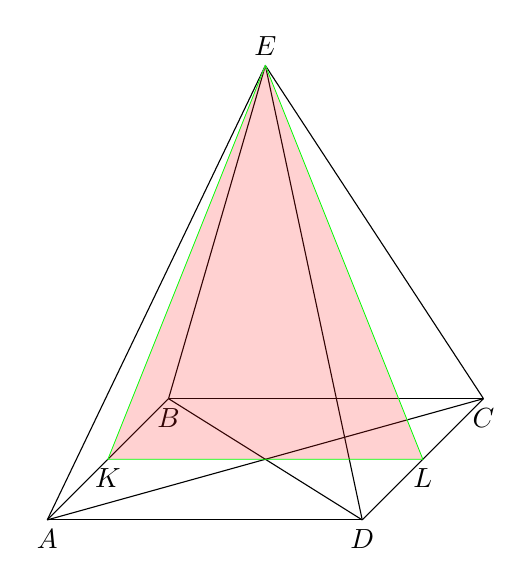
\begin{tikzpicture}
\coordinate (A) at (0,0,4);
\coordinate (B) at (0,0,0);
\coordinate (C) at (4,0,0);
\coordinate (D) at (4,0,4);
\coordinate (E) at (2,5,2);
\coordinate (K) at (0,0,2);
\coordinate (L) at (4,0,2);
\draw (A) -- (B) node [below] {$B$};
\draw (A) -- (D) node [below] {$D$};
\draw (C) -- (A) node [below] {$A$};
\draw (B) -- (C) node [below] {$C$};
\draw (C) -- (D);
\draw (A) -- (E) node [above] {$E$};
\draw (E) -- (B);
\draw (E) -- (C);
\draw (E) -- (D);
\draw (B) -- (D);
\draw[line width = 0.1mm, white](E) -- (K) node [below,black] {$K$};
\draw[line width = 0.1mm, white](E) -- (L) node [below,black] {$L$};
\filldraw[draw = green, line width = 0.1mm, fill=red!90, fill opacity=0.2 ] (E) -- (L) -- (K) -- cycle;
\end{tikzpicture}
\end{document}